\RequirePackage{ifpdf}
\ifpdf
	\documentclass[11pt,oneside,a4paper,pdftex]{article}   %two-page printing
\else
	\documentclass[11pt,twoside,a4paper,dvips]{article}   %two-page printing
\fi

%\documentclass[a4paper, 12pt]{article}
\addtolength{\hoffset}{-1.9cm}
\addtolength{\voffset}{-1.9cm}
\addtolength{\textwidth}{+3.8cm}
\addtolength{\textheight}{+3.8cm}
\usepackage[latin1,utf8]{inputenc}
\usepackage[czech]{babel}
\usepackage{icomma} % ceska desetinna carka
\usepackage{csquotes}
\usepackage{listings}
\usepackage{amsmath}
\usepackage{amsthm}
\usepackage{amsfonts}
\usepackage{mathrsfs}
%\usepackage[T1]{fontenc}
\ifpdf
	\usepackage[pdftex]{graphicx} % dvips or pdftex
\else
	\usepackage[dvips]{graphicx} % dvips or pdftex
\fi
\usepackage[center]{subfigure}
\usepackage{amsfonts}
\usepackage[dvips]{color}               %for using colors
%\usepackage{showframe}                 %zobrazuje okraje stranky
\usepackage[justification=justified,hang]{caption}
\usepackage{textpos}
\usepackage{url}
%\usepackage{fancybox}
\usepackage{verbatim}
\usepackage{fj}
\ifpdf
	\usepackage[pdftex,unicode,colorlinks]{hyperref}
\else
	\usepackage[unicode]{hyperref}
\fi


\title{A4M33TDV Homework H2: "Compute height ratio" (p. 46)}
\date{18. 10. 2011}
\author{Filip Jareš}

\begin{document}
\selectlanguage{english}

\maketitle

\section{Assignment}

\noindent What is the ratio of heights of Building A to Building B?

\paragraph{Hints}

\begin{enumerate}
		\item What are the properties of line $h$ connecting the top of Buiding B with the point $m$
			at which the horizon is intersected with the line $p$ joining the foots of both buildings? [1~point]
		\item How do we actually get the horizon $n_\infty$ ? [1~point]
		\item What tool measures the length? [formula = 1~point]
\end{enumerate}


\begin{figure}[htb]
	\centering
	\subfigure[] {
		\fbox{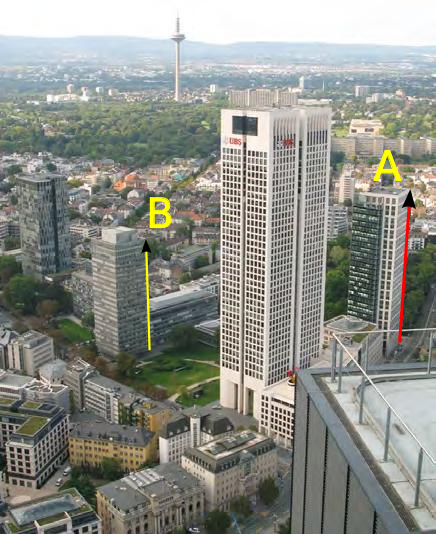
\includegraphics[width=6.5cm]{buildings-with_arrows.jpeg}}
		\label{photo}
	}
	\subfigure[] {
		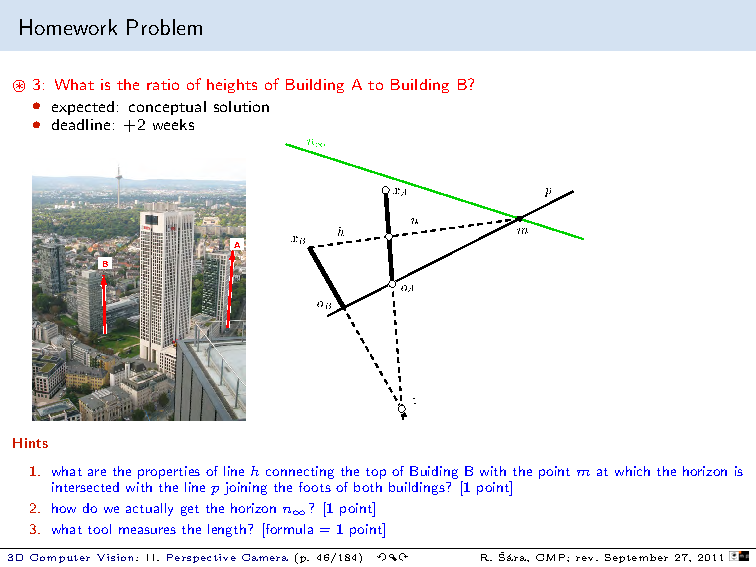
\includegraphics[width=6.5cm,clip=true,trim=4.5cm 2cm 3cm 2cm]{pg_0019.pdf}
		\label{scheme}
	}
	\caption{}
	\label{buildings}
\end{figure}

\section{Conceptual solution}

Let us denote points and lines in the \emph{image} using lowercase letters (according to the figure \ref{scheme})
and corresponding points and lines in the 3D \emph{world} using uppercase letters.

\paragraph{Properties of line $h$} The line $h$ is a horizontal line (assuming that line
$P$ is horizontal in the scene (in 3D) and that line $n_\infty$ is vanishing line of horizontal planes).

\paragraph{Getting the horizon} We can get the horizon line $n_\infty$ by connecting two vanishing points
of two different sets of horizontal parallel lines. (For example edges and railings on the roof of the building
in the foreground can be used for this purpose.)

\paragraph{Measuring length} Heights of buildings A and B can be compared when we take into account
point $u$ (intersection of horizontal line $h$ with line representing the building A, see figure \ref{scheme}).
If $u \equiv x_A$, then heights of both buildings are the same. If $|x_A\,o_A| < |u\,o_A|$ holds for distances, then
the building A is lower than building B. If $|x_A\,o_A| > |u\,o_A|$ holds, then building A is the higher one.

One can use cross ratio of points $[x_A, u, o_A, z] = [X_A, U, O_A, Z]$ to express the ratio of heights of both buildings.
The point $z$ used in the cross ratio is the vanishing point of vertical lines. We can cancel out distances
of finite points $X_A$ and $U$ to the infinite point $Z$ in the cross ratio of \emph{world} points. Therefore
we get following formula for the ratio of height of building A ($l_A$) and building B ($l_B$):

\begin{equation}
	\label{eq}
	\frac{l_A}{l_B} = \frac{|X_A\,O_A|}{|U\,O_A|} = \frac{|X_A\,O_A|\,|U\,Z|}{|X_A\,Z|\,|U\,O_A|} = \frac{|x_A\,o_A|\,|u\,z|}{|x_A\,z|\,|u\,o_A|}.
\end{equation}

\section{Numerical soluition}

I tried to determine relevant vanishing points, the horizon line and the intersection $u$ of the horizontal line
with the line representing the building A and using the formula (\ref{eq}) I have obtained following result for
the given picture (figure \ref{photo}):

		$$ \frac{l_A}{l_B} = 1.52. $$
	


\end{document}

